\documentclass[11pt]{article}



% unnecessary commands
\newcommand{\etal}{\textit{et~al.}\xspace}
\newcommand{\eg}{\textit{e.g.},\xspace}
\newcommand{\ie}{\textit{i.e.},\xspace}
\newcommand{\aka}{\textit{a.k.a.},\xspace}
\newcommand{\etc}{etc.\xspace}
\newcommand{\cf}{cf.\/~}
\newcommand\figref[1]{Figure~\ref{#1}}
\newcommand\algrefNew[1]{Algorithm~\ref{#1}}
\newcommand\tabref[1]{Table~\ref{#1}}
\newcommand\secref[1]{Section~\ref{#1}}
\newcommand\equref[1]{Equation~(\ref{#1})}
\newcommand\defref[1]{Definition~\ref{#1}}
\newcommand{\fakeparagraph}[1]{\vspace{1mm}\noindent\textbf{#1.}}


\newcommand{\FNew}{\mathcal{F}}
\newcommand{\D}{\mathcal{D}}
\newcommand{\Q}{\mathcal{Q}}
\newcommand{\T}{\mathcal{T}}
\newcommand{\M}{\mathcal{M}}
\newcommand{\obj}{o}

\ifodd 1
\newcommand{\rev}[1]{{\color{blue}#1}} %revise of the text
\newcommand{\zeng}[1]{{\color{brown}#1}} %revise of the text
\newcommand{\TODO}[1]{{\color{red}{\textbf{TODO}:{ #1}}}}
\else
\newcommand{\rev}[1]{#1}
\newcommand{\zeng}[1]{#1}
\newcommand{\TODO}[1]{}
\fi

\title{Federated Computing: Query, Learning, and Beyond}

\author{Yongxin Tong$^{\dagger}$
\hspace{1em} Yuxiang Zeng$^{\dagger,\ddagger}$
\hspace{1em} Zimu Zhou$^{\sharp}$
\hspace{1em} Boyi Liu$^{\dagger}$
\hspace{1em} Yexuan Shi$^{\dagger}$\\
\hspace{1em} Shuyuan Li$^{\dagger}$
\hspace{1em} Ke Xu$^{\dagger}$
\hspace{1em} Weifeng Lv$^{\dagger}$
\\
$^{\dagger}$ State Key Laboratory of Software Development Environment,\\
Beijing Advanced
Innovation Center for Future Blockchain and Privacy Computing, \\
School of Computer Science, Beihang University, Beijing, China \\
\texttt{\small\{yxtong,turf1013,liuby,skyxuan,lishuyuan,kexu,lwf\}@buaa.edu.cn} \\
$^{\ddagger}$ The Hong Kong University of Science and Technology, Hong Kong SAR, China \\
$^{\sharp}$ City University of Hong Kong, Hong Kong SAR, China \hspace{1em} \texttt{\small zimuzhou@cityu.edu.hk}
}


\begin{document}
\maketitle

\begin{abstract}\label{sec:abstract}
Big data has played an important role in the development of the economy.
However, the ``data isolation'' problem largely hinders its full potential.
To solve this problem, it is crucial to enable collaborative computing among multiple data sources.
Federated computing, a new collaborative computing paradigm that keeps the raw datasets decentralized, has emerged as a hot research topic in both databases and artificial intelligence.
This paper introduces the concepts of federated computing, reviews recent topics, which include ``federated queries'' and ``federated learning'', and discusses the future trends.

\end{abstract}

\section{Introduction}\label{sec:introduction}
In the era of big data, governments, organizations, companies, and individuals rely heavily on data analysis for decision-making.
However, the ``data isolation’’ problem remains a major bottleneck for big data analysis.
As the name implies, data is stored as islands among multiple data owners, which seriously hinders the sharing and circulation of big data.
For example, medical big data can be used to build accurate machine learning models for disease prediction and diagnosis.
However, patients' data, \eg medical examination results, may distribute across multiple autonomous hospitals, which hinders joint analysis due to privacy concerns.
Another example is the smart city applications with big spatiotemporal data.
In these applications, the spatiotemporal data are distributed in multiple platforms, \eg taxi and ride data on multiple travel platforms, meal data on the catering platform, and cell tower data on telecommunications operation service providers. Due to the privacy concerns, it is difficult to collect these data directly, which hinders the rapid response of smart city applications.
Therefore, how to break the data isolation and unite multiple data owners for computation is crucial to strengthen the circulation of data and the development of the big data industry.

To break the data isolation dilemma, ``federated computing'' is proposed as a new collaborative computing paradigm, where multiple data owners are united as a data federation and process collaborative computing while keeping the raw data locally at each data owner~\cite{Yongxin-DBLP:journals/tist/YangLCT19,Yongxin-ref_bater2017smcql,Yongxin-DBLP:conf/sigmod/BharadwajC22}.
Its idea is to push the computation on raw data to the data owners, while only summary information from the raw data is communicated back to the server for secure aggregation.

\fakeparagraph{Challenges}
Federated computing mainly faces three challenges.
\textit{(i) Privacy.}
Federated computing poses new privacy constraint, \ie the raw data of each data owner is kept locally, while allowing collaborative computing among data owners.
\textit{(ii) Efficiency.}
Since privacy and security constraints often introduce extra communication and computation, it is important to comply with these constraints while allowing high-efficiency computing.
\textit{(iii) Effectiveness.}
As the data of multiple data owners may not be independent and identically distributed (non-IID), how to conduct accurate analysis in presence of data heterogeneity is also a challenge.

\fakeparagraph{Milestones}
Two hot topics in current federated computing are ``federated queries" and ``federated learning".
\begin{itemize}
    \item
    The federated queries indicate that the data federation should support secure queries over multi-party data owners.
    It serves as the basis of federated computing.
    Several data federation systems have been proposed to support various federated queries, such as \textsf{SMCQL}~\cite{Yongxin-ref_bater2017smcql}, \textsf{Hu-Fu}~\cite{Yongxin-ref_tong2022hu}, \textsf{FedGraph} \cite{Yongxin-DBLP:journals/pvldb/YuanMWZW21}, which are designed for relational, spatial, and graph queries, respectively.
    \item
    Upon a data federation, machine learning algorithms can be further implemented to support upper-layer applications.
    Such algorithms are often known as ``federated learning''.
    For example, \textsf{FedAvg} \cite{Yongxin-DBLP:conf/aistats/McMahanMRHA17} is one of the most popular federated learning algorithms, and there have been extensions to more generic frameworks \cite{Yongxin-DBLP:journals/tist/YangLCT19}.
\end{itemize}

\fakeparagraph{Roadmap}
In the rest of this paper, we first introduce the basic concepts and general framework of federated computing in \secref{sec:concept}.
Then, we review the related work on federated queries (\secref{sec:data}) and federated learning (\secref{sec:learning}), respectively.
Finally, we summarize the future directions in \secref{sec:future} and conclude in \secref{sec:conclusion}.

\section{Basic Concepts and General Framework}\label{sec:concept}
This section introduces the basic concepts and general framework of federated computing in \secref{sec:concept-def} and \secref{sec:concept-framework}, respectively.

\subsection{Basic Concepts of Federated Computing}\label{sec:concept-def}

In the following, we introduce the key concepts in federated computing
and the problem statement.

\fakeparagraph{Data Federation}
Federated computing is performed over a special data system, \ie \textit{data federation}.

\begin{definition}[Data Federation]\label{def:fed-data}
A data federation $\FNew$ is a federation of local datasets $\{\D_1, \D_2, \cdots, \D_m\}$ held by $m$ data owners, where each local dataset $\D_i$ has $n_i$ objects $\{\obj_1, \obj_2, \cdots, \obj_{n_i}\}$ and each object $\obj_j$ has $k_j$ attributes $\{x_1, x_2, \cdots, x_{k_j}\}$.
Then, the (virtual) database of this data federation is denoted by the union of these local datasets, \ie $\D = \D_1 \cup \D_2 \cup \cdots \cup \D_m$.
\end{definition}

When local datasets are data silos of data owners like enterprises and organizations,
we call this setting ``cross-silo''.
By contrast, when data owners are individuals like mobile phone users or edge device users,
we call this setting ``cross-device''.
Accordingly, the application settings of federated computing can be categorized into \textit{cross-silo} and \textit{cross-device} \cite{Yongxin-DBLP:journals/ftml/KairouzMABBBBCC21}.
For example, a data federation system was built to answer collaborative queries over clinical data across organizations under the cross-silo setting \cite{Yongxin-science2016A}, while Google allowed their mobile users to jointly train language models under the cross-device setting \cite{Yongxin-DBLP:conf/aistats/McMahanMRHA17}.

\begin{figure}[t]
	\centering
	\begin{subfigure}[Horizontal data federation]{
		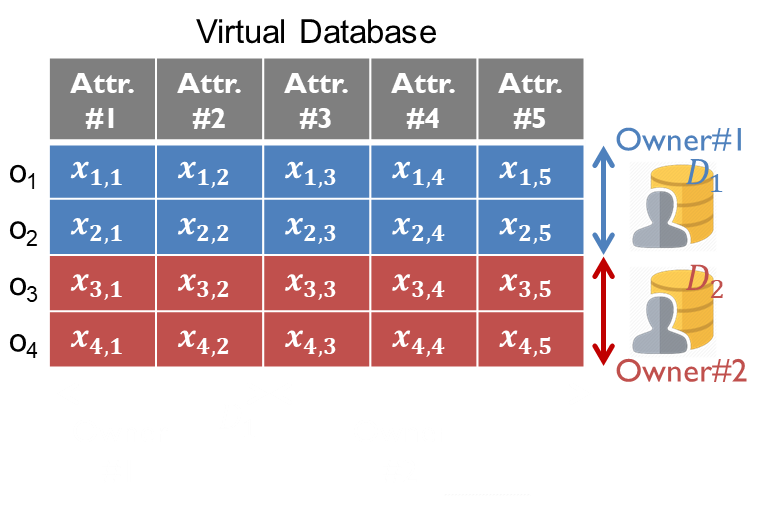
\includegraphics[width=0.52\textwidth]{submissions/YongxinTong/fig/horizontal-partition.png}
		\label{fig:horizontal-data-partition}
    }
	\end{subfigure}
	~
	\begin{subfigure}[Vertical data federation]{
		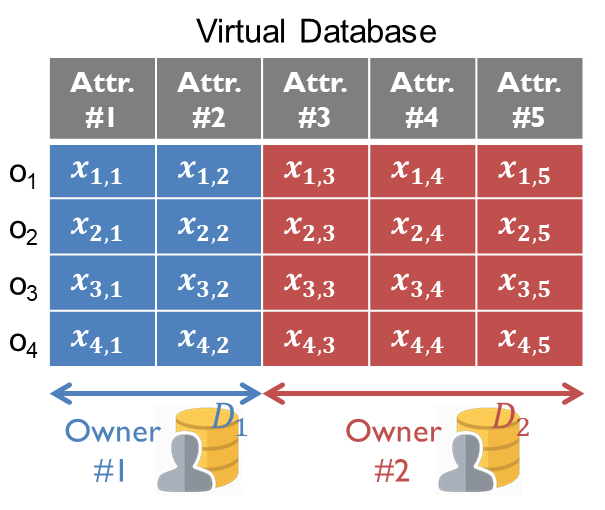
\includegraphics[width=0.42\textwidth]{submissions/YongxinTong/fig/vertical-partition.png}
		\label{fig:vertical-data-partition}
    }
	\end{subfigure}
	\caption{Two ways for data owners' local datasets to integrate into a data federation, including (a) horizontal data federation and (b) vertical data federation.}\label{fig:data-partition}
\end{figure}

\fakeparagraph{Data Integration Mode}
On the other hand, from the perspective of how the local datasets are integrated into the virtual database,
a data federation can be categorized into \textit{horizontal data federation} (\aka horizontally partitioned data \cite{Yongxin-DBLP:conf/kdd/VaidyaC02}) and \textit{vertical data federation} (\aka vertically partitioned data \cite{Yongxin-DBLP:journals/tkde/KantarciogluC04}).
As shown in \figref{fig:data-partition}, in a horizontal data federation, each data owner has a disjoint subset of rows in the virtual database. By contrast, in a vertical data federation, each data owner has a disjoint subset of columns in the virtual database.
Both types are commonly seen in existing literature \cite{Yongxin-DBLP:journals/tist/YangLCT19}.

\fakeparagraph{Problem Statement} A formal definition of federated computing is as follows.

\begin{definition}[Federated Computing]\label{def:fed-compute}
	Given a data federation $\FNew$ of $m$ data owners $\{\D_i\}$ and a computing task $\T(\D)$ over the (virtual) database $\D=\cup_{i=1}^{m}{\D_i}$,
	a federated computing algorithm aims to compute the result of $\T(\D)$ while satisfying the following constraints:
	\begin{itemize}
		\item \textbf{Autonomous Constraint}: any data owner does not share his raw data to others.
		\item \textbf{Security Constraint}: during the computation, except for the result, any sensitive data of a data owner cannot be leaked to others.
	\end{itemize}
\end{definition}

In \defref{def:fed-compute}, the autonomous constraint is aligned with real-world scenarios,
since a data owner would like to autonomously manage his local dataset.

\fakeparagraph{Attacker Models}
The security constraint is due to the concern of privacy attacks, which are commonly seen nowadays and can be categorized into two kinds, \textit{semi-honest adversary} and \textit{malicious adversary}.
\begin{itemize}
	\item \textbf{Semi-honest Adversary}: a semi-honest adversary will honestly follow the specified computation procedure,
	but may attempt to infer sensitive data of data owners in the meantime.
	\item \textbf{Malicious Adversary}: a malicious adversary may arbitrarily deviate from the specified computation procedure to infer sensitive data.
\end{itemize}

\subsection{General Framework for Federated Computing}\label{sec:concept-framework}

Solutions to federated computing can be summarized into a two-phase general framework. The \textit{main idea} of this general framework is as follows.
\begin{itemize}
	\item \textbf{Local Computation.} First, motivated by the idea of computation pushdown, a federated computing task is decomposed into several computing tasks over the local datasets, and hence data owners can locally compute their partial results.
	\item \textbf{Secure Computation.} After that, a well-designed protocol is performed across data owners to derive the final result based on their partial results in a privacy-preserving manner. Finally, the final answer will be returned to the service user.
\end{itemize}

The federated computing task $\T$ in existing work can be mainly classified into two kinds, \textit{federated query} and \textit{federated learning}, which will be elaborated later in \secref{sec:data} and \secref{sec:learning}, respectively.
To evaluate the performance of solutions to federated queries and federated learning, commonly-used metrics include result accuracy, time efficiency, communication cost, \etc

\newcommand{\SMCQL}{\textsf{SMCQL}\xspace}
\newcommand{\SAQE}{\textsf{SAQE}\xspace}
\newcommand{\Shrinkwrap}{\textsf{ShrinkWrap}\xspace}
\newcommand{\HuFu}{\textsf{Hu-Fu}\xspace}
\newcommand{\Conclave}{\textsf{Conclave}\xspace}
\newcommand{\Senate}{\textsf{Senate}\xspace}
\newcommand{\Opaque}{\textsf{Opaque}\xspace}

\section{Federated Queries}\label{sec:data}

In this section, we introduce how to process federated queries over a data federation.
Specifically, we first present the key concepts and main workflow of federated queries in \secref{sec:data-overview}.
Then, we introduce the techniques of processing federated queries from three aspects,
query rewrite (\secref{sec:data-rewrite}), local queries (\secref{sec:data-local}), and secure operations (\secref{sec:data-secure}).
Finally, we summarize these studies in \secref{sec:data-summary}.

\subsection{Overview}\label{sec:data-overview}

\fakeparagraph{Problem Statement}
Based on \defref{def:fed-query}, we introduce the formal definition of federated queries as follows.

\begin{definition}[Federated Query]\label{def:fed-query}
	Given a data federation $\FNew$ of $m$ data owners $\{\D_i\}$ and a query request $\Q$ over the (virtual) database $\D=\cup_{i=1}^{m}{\D_i}$,
	a federated query aims to retrieve the result $\Q(\D)$ while satisfying the autonomous constraint and security constraint in \defref{def:fed-compute}.
\end{definition}

For an exact query $\D$, the answer $\Q(\D)$ should be equal to the (exact) result under an ideal case when all local datasets $\{\D_i\}$ have been integrated into one database $\D$.
By contrast, for an approximate query $\D$, the answer $\Q(\D)$ may be different from the (approximate) result under such a case.
Instead, an approximation guarantee is often studied to control the result error for approximate queries.

\begin{figure}[t]
\centering
    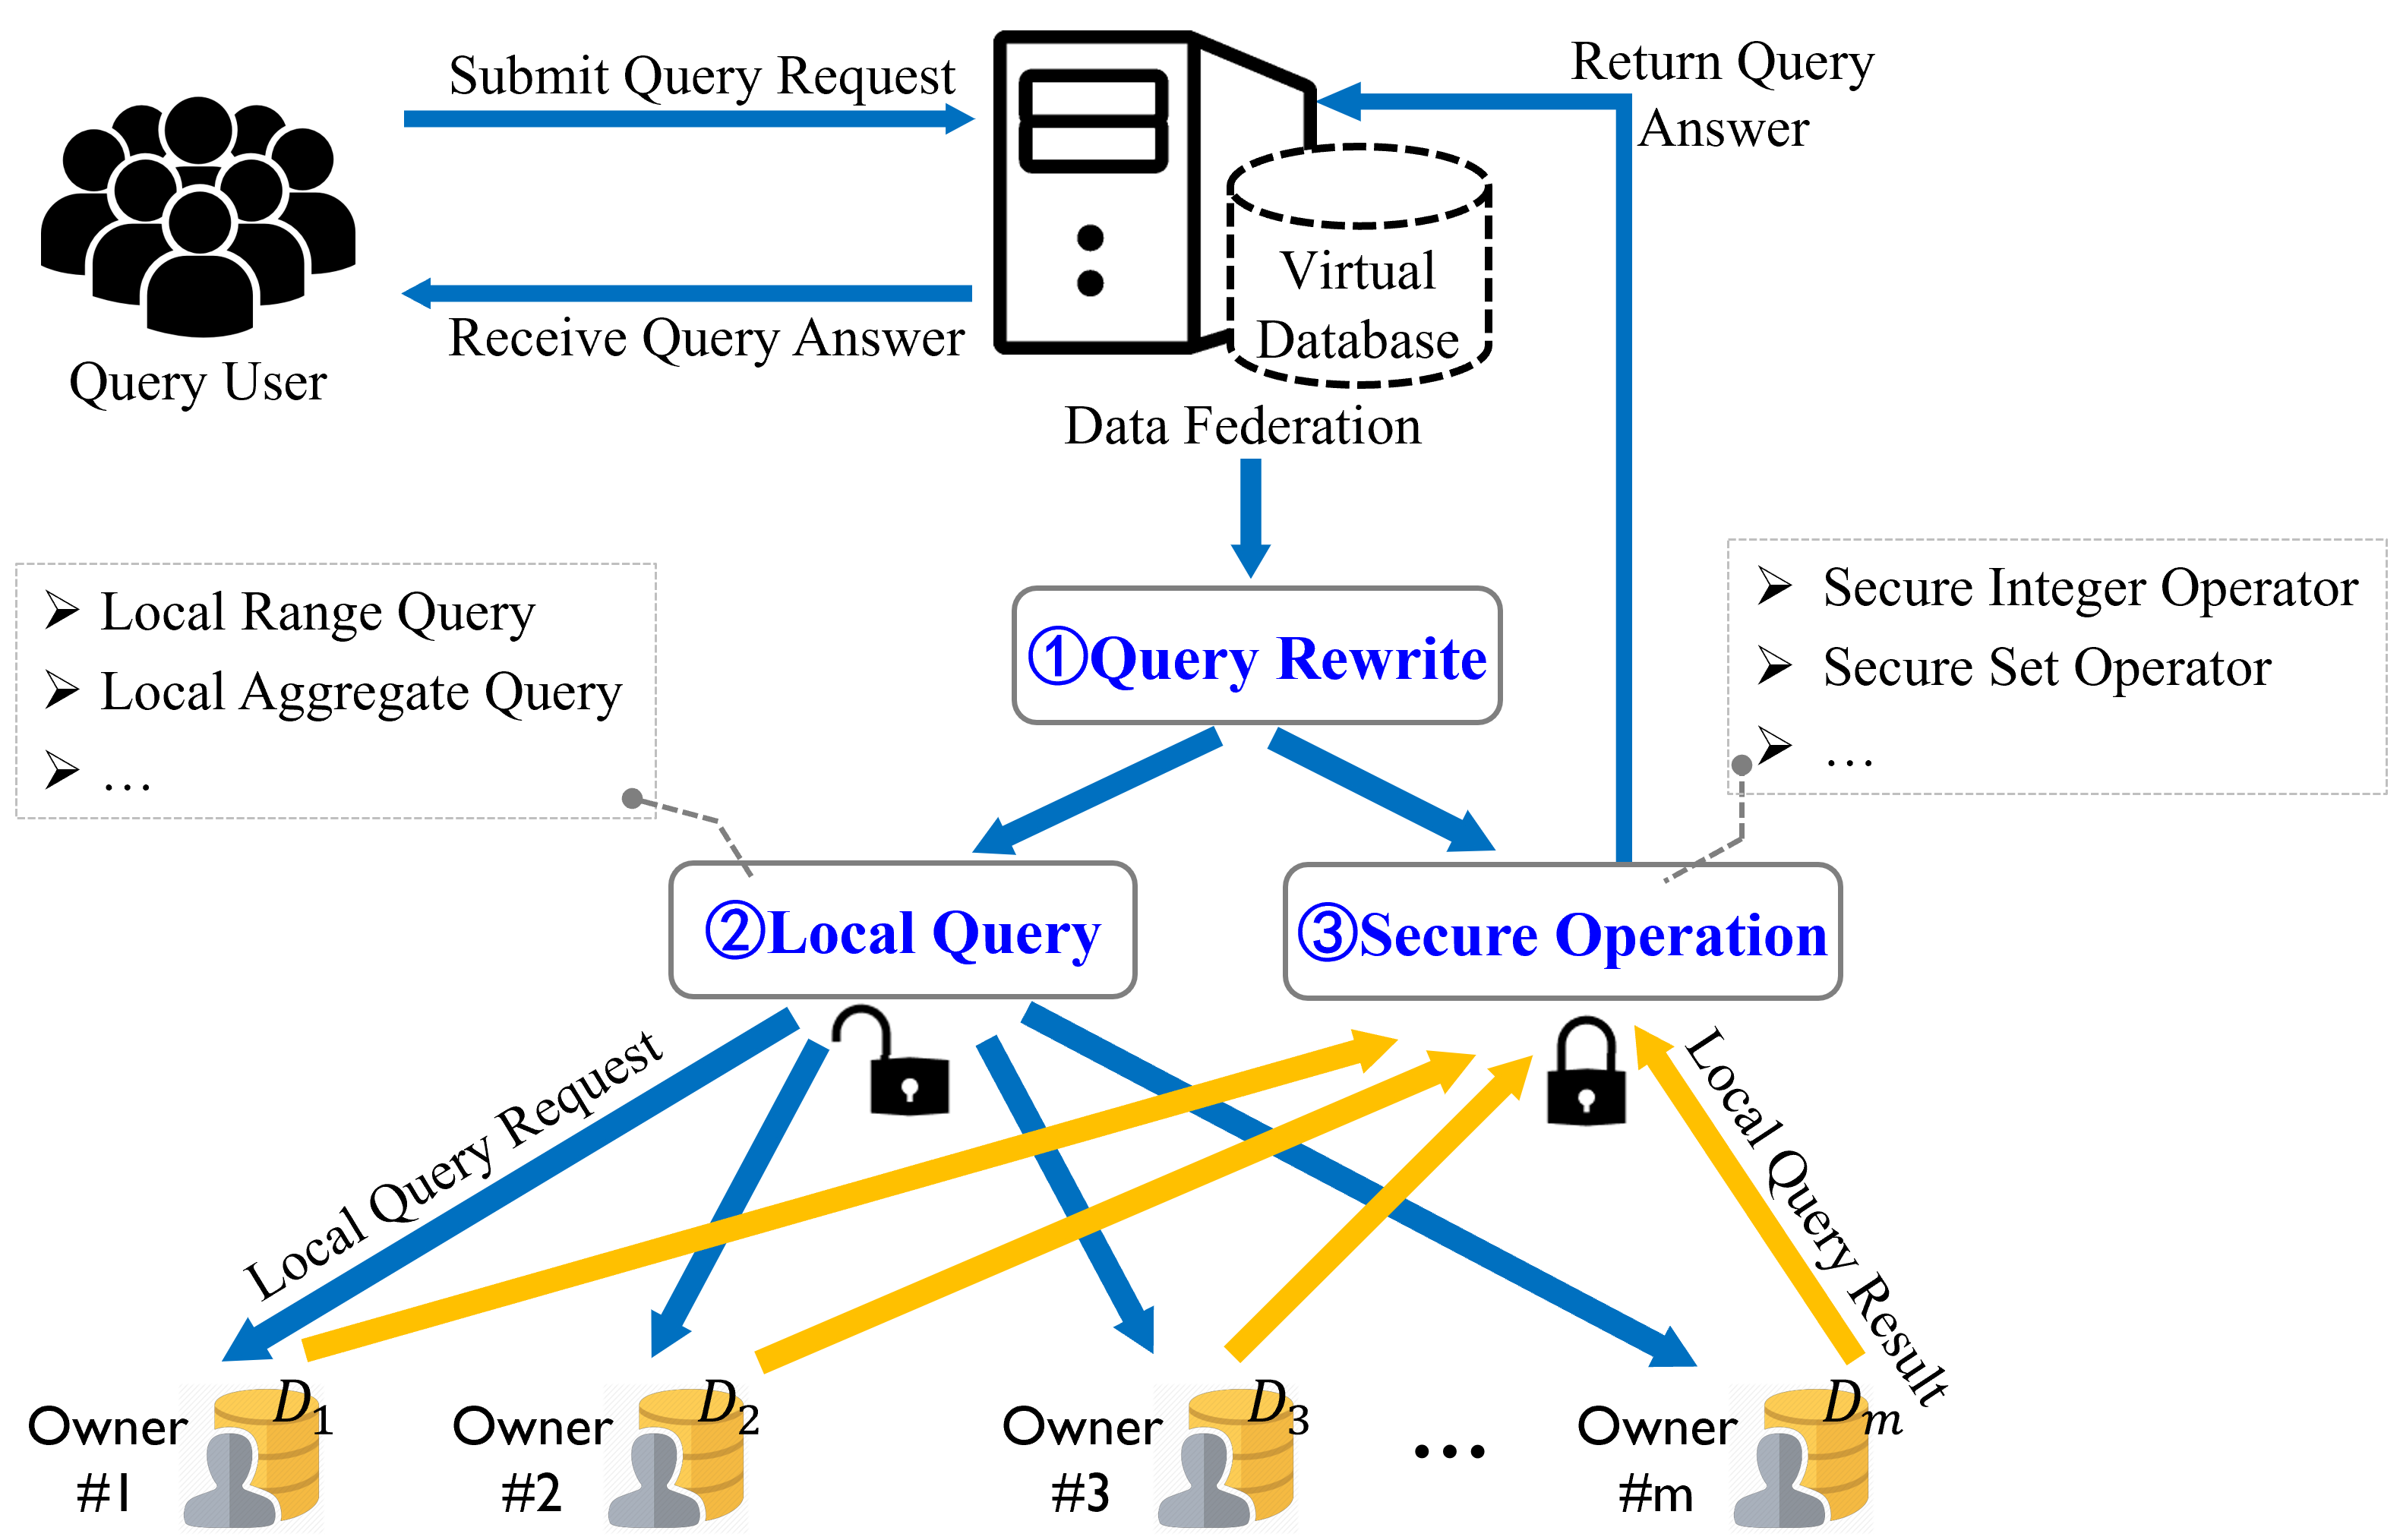
\includegraphics[width=0.8\linewidth]{submissions/YongxinTong/fig/query.png}
	\caption{Workflow of processing federated queries over a data federation.}\label{fig:workflow-query}
\end{figure}

\fakeparagraph{Workflow of Processing Federated Queries}
As shown in \figref{fig:workflow-query}, a service user first submits his query request $\Q$ to the central server (\aka coordinator or broker).
Next, the server parses and rewrites the query $\Q$ to form a series of local queries and secure operations, which is generally aligned with our general framework in \secref{sec:concept-framework}.
Then, the server sends local queries to data owners, and asks them to perform local queries.
When all of them have computed the local results, the server will coordinate these data owners to jointly perform secure operations by following the pre-designed protocols and obtain intermediate results or final results.
The procedure ends after one or multiple rounds of local queries and secure operations, depending on the query type.

Here, we take the federated range counting query over a horizontal data federation as an example.
As shown in \figref{fig:horizontal-data-partition}, data owners in a horizontal data federation hold different rows of the (virtual) table $\D$.
According to the aforementioned workflow, a federated range counting query can be answered by performing a local range counting query over each local dataset $\D_i$ and a secure summation of these partial results across all data owners.

Intuitively, the performance of local queries and secure operations is critical to the performance of federated query processing.
Thus, in the following, we introduce existing techniques for managing data federation from three categories, query rewrite (\secref{sec:data-rewrite}), local queries (\secref{sec:data-local}), and secure operations (\secref{sec:data-secure}).

\subsection{Query Rewrite}\label{sec:data-rewrite}

The \textit{common idea} of query rewriters in federated queries is to use as many local queries and as few secure operations as possible \cite{Yongxin-ref_tong2022hu}.
This is because a secure operation across a large number of data owners is often more time-consuming than local queries that could be naturally sped up by modern database techniques.
Based on this idea, existing query rewriter can be classified into two kinds, \textit{query rewriter via annotating query plan tree} and \textit{query rewriter via customized rule}.

\fakeparagraph{Query Rewriter via Annotating Query Plan Tree}
In this category, after receiving the query request, the coordinator will parse the federated query into a directed acyclic graph (DAG) by using well-known solutions (\eg Apache Calcite \cite{Yongxin-DBLP:conf/sigmod/BegoliCHML18}).
This DAG, which represents the query plan (when data is plaintext), is usually a tree of relational algebraic operations.
After that, the coordinator will traverse the tree bottom-up (or sometimes up-down) to annotate the operations that require extra security protections (\ie secure operations).

Specifically, \SMCQL \cite{Yongxin-ref_bater2017smcql}, a system for processing federated queries, classified the levels of data access into three categories, public, protected, and private attributes.
Here, public attributes are accessed by anyone (\eg the other data owners), and protected attributes could be accessed by the data owner, coordinator, and query user.
By contrast, private value can be only accessed by the data owner himself.
Accordingly, operators in the query plan tree can be categorized into three preservation kinds, \textit{plaintext operators}, \textit{secure operators}, and \textit{prohibitive operators} (\ie three kinds of annotations).
Then, the annotations can be determined by examining the data access levels of its output attributes and considering the most stringent level of its source attributes.
For example, consider the federated top-$k$ query over the attribute ID in the following:
\begin{lstlisting}[language=SQL]
  SELECT ID FROM F ORDER BY ID LIMIT k;
\end{lstlisting}
\begin{enumerate}[label=(\roman*)]
	\item If ID is public, the query plan consists of two plaintext operators, \ie sort and limit $k$ (by ID).
	\item If ID is protected, the aforementioned two operators should be securely executed.
	\item If ID is private, any query plan is prohibitive, since a private output attribute cannot be revealed to the service user.
\end{enumerate}

To further optimize the query plan, Bater \etal \cite{Yongxin-ref_bater2017smcql} proposed a technique called \textit{slicing} with the goal of minimizing the time cost of secure operations.
They aimed to slice the secure operators into ``smaller and more manageable units of computation'' \cite{Yongxin-ref_bater2017smcql}.
For instance, when ID is protected in the above example, one can slice the secure sort into \textit{first} plaintext limit $k$ over each data owner's local dataset and \textit{then} secure sort over the remaining $mk$ IDs,
where $m$ is the number of data owners.
The query rewriters of other systems for federated queries, such as \Shrinkwrap \cite{Yongxin-ref_bater2018shrinkwrap} and \SAQE \cite{Yongxin-ref_bater2020saqe}, followed a similar idea with that of \SMCQL.
The system \Conclave \cite{Yongxin-ref_volgushev2019conclave} considered the scenario that a data owner may permit specific selectively-trusted parties (\eg a government regulator) to access his sensitive attributes and optimized the query rewriter under this assumption.

\fakeparagraph{Query Rewriter via Customized Rule}
Another way is to design customized query decomposition rules for specific query types.
A typical example is the federated $k$-nearest-neighbor ($k$NN) query \cite{Yongxin-ref_tong2022hu} in the spatial data federation.
Although it is a spatial query, its query plan can be referred to that of federated top-$k$ query, as aforementioned.
Unfortunately, the efficiency has been shown to be low in large-scale datasets \cite{Yongxin-ref_tong2022hu}, since a secure sort is very time-consuming.
Thus, Tong \etal \cite{Yongxin-ref_tong2022hu} were motivated to design a novel query plan for federated $k$NN in their system \HuFu.
The \textit{basic idea} is to (1) determine the $k$th nearest distance to the query object by binary search and (2) retrieve the answer by a range query with the radius of the $k$th nearest distance.
Accordingly, the query plan of the first step consists of local range counting queries (with the searching distance) and secure comparison (between the summation of all local counts and threshold $k$),
and the query plan of the second step is the same as that of a federated range query.
Another example is that Wang \etal \cite{Yongxin-ref_wang2021secure} devised an efficient query plan for federated join-aggregate queries.
Their basic idea is to decompose federated join-aggregate queries into semijoins and full joins.

\subsection{Local Query}\label{sec:data-local}

After getting the query plan, the coordinator often sends local queries to data owners prior to the secure operations.
Thus, in the following, we introduce mainstream optimization techniques for processing local queries in a data federation from two aspects, \textit{indexing} and \textit{sampling}.

\fakeparagraph{Optimization By Indexing}
Indexing is usually used to improve the time efficiency of processing local queries.
In particular, local queries in a data federation can be benefited from the recent development of indexing techniques.
In recent years, the \textit{learned index} is one of the most popular indexing techniques in existing literature.
The \textit{main idea} of a learned index is to view the data indexing problem as a machine learning problem that learns the mapping function between the search key and its corresponding location in the storage.
Based on this idea, promising results of lookup queries and range queries over 1-dimensional data have been achieved by 1-dimensional learned indexes, such as RMI~\cite{Yongxin-DBLP:conf/sigmod/KraskaBCDP18}, PGM-index \cite{Yongxin-DBLP:journals/pvldb/FerraginaV20}, ALEX \cite{Yongxin-DBLP:conf/sigmod/DingMYWDLZCGKLK20}, and LIPP~\cite{Yongxin-DBLP:journals/pvldb/WuZCCWX21}.
Multi-dimensional learned indexes have also been devised to support $k$NN queries, such as ZM-Index~\cite{Yongxin-DBLP:conf/mdm/WangFX019}, IF-Index~\cite{Yongxin-DBLP:conf/vldb/0001KH20}, Lisa~\cite{Yongxin-DBLP:conf/sigmod/Li0ZY020}, and RSMI~\cite{Yongxin-DBLP:journals/pvldb/QiLJK20}.
For more details, please refer to the tutorials \cite{Yongxin-DBLP:conf/sigmod/IdreosK19} and experimental work \cite{Yongxin-DBLP:journals/pvldb/MarcusKRSMK0K20}.

\fakeparagraph{Optimization By Sampling}
Another way of optimizing local queries is to use sampling that may sacrifice result accuracy for efficiency.
Such techniques in federated queries can be classified into two kinds, \textit{sampling data owners} and \textit{sampling data records}.
\begin{itemize}
	\item \textbf{Sampling Data Owners.}
	The \textit{main idea} of sampling data owners is to utilize the local results of the sampled data owners to estimate the local results of the others.
	For example, to process federated range aggregation queries over a spatial data federation, Shi \etal \cite{Yongxin-ref_shi2021efficient} used the result of a local range aggregation query over one data owner to derive an unbiased estimation of the others, where local datasets are identically and independently distributed (IID).
	To break the IID assumption and tackle the non-IID scenario, they proposed a grid index to decompose the underlying spatial area into small enough regions and achieve a more fine-grained approximation by aggregating the estimation result in each region.
	They also proved that the estimated result can be closed enough to the exact result with high probability \cite{Yongxin-ref_shi2021efficient}.
	
	\item \textbf{Sampling Data Records.}
	The \textit{main idea} of sampling data records is to use the results of sampled data records to estimate the results of all data records within a local dataset.
	For example, Bater \etal \cite{Yongxin-ref_bater2020saqe} have applied three sampling strategies in their system for \SAQE federated queries, \ie uniform sampling, stratified sampling, and distinct sampling, which are well-known sampling strategies in approximate query processing \cite{Yongxin-DBLP:conf/sigmod/ChaudhuriDK17}.
	Shi \etal \cite{Yongxin-ref_shi2021efficient} adopted level sampling to achieve load balancing when performing local queries over unbalanced local datasets. Notice that, different from a traditional distributed database system,
	data partition or re-partition, which is a commonly-used technique for load balancing, is not allowed in a data federation, since each data owner would like to autonomously manage his own data.
\end{itemize}

In general, the strategy of sampling data owners is orthogonal to that of sampling data records.
The technical challenge of jointly using both sampling strategies is how to make a proper trade-off between result accuracy and efficiency, especially under the non-IID scenario.

\subsection{Secure Operation}\label{sec:data-secure}

After getting the results of local queries, secure operations are often invoked to jointly compute an intermediate result or a final result across all data owners and guarantee that no sensitive information (\eg private attributes) of one data owner is leaked to others during this collaborative computation.
We introduce existing solutions to secure operations when processing federated queries from two aspects, \ie
\textit{secure multi-party computation (SMC) based solution} and \textit{differential privacy (DP) based optimization}.

\fakeparagraph{SMC based Solution}
SMC has been studied for over three decades in academia \cite{Yongxin-DBLP:journals/cacm/Lindell21}.
The goal of SMC is to jointly compute some functions based on the private inputs of data owners in the data federation.
Moreover, SMC also requires that (1) the result should be accurate and (2) no information can be leaked except for that derived from the output, which is coincident with the constraints of federated queries in \defref{def:fed-query}.
Thus, SMC is a prevalent method to implement secure operations.

Specifically, the systems for federated queries, \SMCQL \cite{Yongxin-ref_bater2017smcql} and \Shrinkwrap \cite{Yongxin-ref_bater2018shrinkwrap}, used a general-purpose programming framework of SMC (\aka SMC compilers), called ObliVM \cite{Yongxin-DBLP:conf/sp/LiuWNHS15}.
ObliVM mainly combines two well-known techniques in SMC, \ie Garbled Circuits (GC) \cite{Yongxin-DBLP:conf/focs/Yao82b} and Oblivious RAM (ORAM) \cite{Yongxin-DBLP:journals/jacm/GoldreichO96}.
GC can securely compute most of operations over two data owners, and ORAM is a safe memory abstraction to safely store the intermediate results of GC without leaking any information about the data access pattern.
Other SMC compilers, such as Obliv-C \cite{Yongxin-DBLP:journals/iacr/ZahurE15} and Sharemind \cite{Yongxin-DBLP:conf/esorics/BogdanovLW08}, are used in \Conclave \cite{Yongxin-ref_volgushev2019conclave} to support two or three data owners.
The other studies, such as \cite{Yongxin-ref_tong2022hu} and \cite{Yongxin-dasfaa23aknn}, adopted customized SMC protocols to support specific operations, which could potentially improve the efficiency.
Different from above systems, which assumed semi-honest adversaries, \Senate \cite{Yongxin-DBLP:conf/uss/PoddarKYDPH21} optimized a GC-based SMC protocol \cite{Yongxin-DBLP:conf/ccs/WangRK17a} to protect the security even with malicious data owners.

\fakeparagraph{DP based Optimization}
Differential privacy (DP) \cite{Yongxin-ref_li2016differential} is the state-of-the-art privacy protection technique to theoretically guarantee that one can hardly re-construct the database based on the query results by DP.
In existing studies for federated queries, DP can be used to further improve the efficiency of secure operations by SMC.
For example, \Shrinkwrap \cite{Yongxin-ref_bater2018shrinkwrap} adopted DP to remove quite a few dummy tuples from the intermediate result in ORAM while still protecting the data access pattern.
\SAQE \cite{Yongxin-ref_bater2018shrinkwrap} used DP to hide the true cardinality of data records when performing oblivious sampling and perturb the query result.
\HuFu \cite{Yongxin-ref_tong2022hu} applied DP to speed up the time efficiency of secure comparison with the threshold $k$ when processing federated $k$NN queries.

Beyond the above techniques, trusted hardware enclaves, such as Intel SGX \cite{Yongxin-DBLP:journals/fcsc/ZhengWWFSLZ21}, can be also used to implement secure operations in the system \Opaque \cite{Yongxin-DBLP:conf/nsdi/ZhengDBPGS17}.

\begin{table}[t]
\centering
\caption{Comparison of existing systems for federated queries}\label{tab:data-federation-compare}
\begin{tabular}{cccccc}
\toprule
System & Data Type & \begin{tabular}[c]{@{}c@{}}Data Integration\\ Mode\end{tabular} & Attacker Model & Data Size & \#(Data Owner) \\
\midrule
\SMCQL \cite{Yongxin-ref_bater2017smcql}       & Relational & Horizontal   & Semi-honest & $\le$1K   &  $\le$2\\
\Shrinkwrap \cite{Yongxin-ref_bater2018shrinkwrap}  & Relational & Horizontal   & Semi-honest & $\le$40K  &  $\le$2\\
\SAQE \cite{Yongxin-ref_bater2020saqe}              & Relational & Horizontal   & Semi-honest & $\le$500K &  $\le$2\\
\Conclave \cite{Yongxin-ref_volgushev2019conclave}  & Relational & Horizontal/Vertical   & Semi-honest & $\le$1B   &  $\le$3\\
\HuFu \cite{Yongxin-ref_tong2022hu}                 & Spatial    & Horizontal   & Semi-honest & $\le$1B   &  $\le$10\\
\Senate \cite{Yongxin-DBLP:conf/uss/PoddarKYDPH21}  & Relational & Horizontal   & Malicious   & $\le$160K &  $\le$16 \\
\Opaque \cite{Yongxin-DBLP:conf/nsdi/ZhengDBPGS17}  & Relational & Vertical     & Malicious   & $\le$1M   &  $\le$5\\
\bottomrule
\end{tabular}
\end{table}
\subsection{Discussion}\label{sec:data-summary}

\tabref{tab:data-federation-compare} summarizes the representative work on federated queries, and we have the following observations. First, most of the existing systems for federated queries concern more about semi-honest adversaries than malicious adversaries, although considering malicious adversaries are more challenging. Second, most of these studies focused on the horizontal data federation, while vertical data federation had less attention. Finally, the scalability of existing solutions is sometimes not large enough, especially when processing federated join queries.

\section{Federated Learning}\label{sec:learning}

In this section, we introduce how to perform federated learning over a data federation.
Specifically, we first present the problem statement and main workflow in \secref{sec:learning-overview}.
Then, we introduce the mainstream solutions to federated learning from two aspects,
local training (\secref{sec:learning-local}) and secure aggregation (\secref{sec:learning-secure}).
Finally, we make discussions in \secref{sec:learning-discussion}.

\subsection{Overview}\label{sec:learning-overview}

\fakeparagraph{Problem Statement} Federated learning (FL) was first proposed by Google in 2016 for language prediction tasks \cite{Yongxin-DBLP:conf/aistats/McMahanMRHA17}. The \textit{main idea} of federated learning is to train a global model in collaboration with different data owners while preserving the privacy of their local data. The definition of federated learning is as follows.

\begin{definition}[Federated Learning]\label{def:fed-learning}
Given a data federation $\FNew$ of $m$ data owners (\aka clients) $\{\D_i\}$ and a computing task of training a learning model $\M$ over the (virtual) database $\D=\cup_{i=1}^{m}{\D_i}$, a federated learning algorithm aims to collaboratively train the learning model $\M(\D)$ on the data federation and make the accuracy of $\M(\D)$ close to that of the model $\M$ that directly trains over the virtual database, while satisfying the autonomous constraint and security constraint in \defref{def:fed-compute}.
\end{definition}

\fakeparagraph{Taxonomy}
Federated learning algorithms can be categorized into three kinds,
\textit{horizontal federated learning}, \textit{vertical federated learning}, and \textit{federated transfer learning} \cite{Yongxin-DBLP:journals/tist/YangLCT19} from the perspective of data integration mode across data owners.

\begin{itemize}
    \item \textbf{Horizontal/Vertical Federated Learning.}
    Horizontal/vertical federated learning is named after the data integration mode (\aka data partition mode) in a data federation as shown in \figref{fig:data-partition}. Notice that, for supervised learning tasks, all data owners' datasets in horizontal federated learning have labels, while only one of them in vertical federated learning has labels.
    \item \textbf{Federated Transfer Learning.}
	Federated transfer learning denotes the scenario where two data owners have different samples and feature spaces in the same time. In other words, federated transfer learning enables one data owner to make use of data from another data owner, although there is only little intersection between the feature spaces of their datasets.
\end{itemize}

\fakeparagraph{Workflow of Federated Learning}
According to the general framework of federated computing in \secref{sec:concept-framework}, the workflow of federated learning algorithms is as follows.
In the procedure of federated learning, the server first initializes a global model and distributes the global model to selected data owners. Each selected data owner then trains his local model through the local loss function and uploads his local model to the server. The server securely aggregates all the uploaded local models into the global model. Finally, the above steps are repeated until convergence.

\fakeparagraph{A Case Study: \textsf{FedAvg}}
One representative work in federated learning is \textsf{FedAvg} \cite{Yongxin-DBLP:conf/aistats/McMahanMRHA17}, which supports training several machine learning models, such as MLP, CNN and LSTM, in a data federation.
Here, we take training a CNN model as an example to explain the aforementioned workflow of federated learning. After the server distributes the global model, data owners train their local CNN models with stochastic gradient descent (SGD).
When the local training ends, data owners will upload the parameters of their local CNN models to the server.
Then, the server aggregates all the received model parameters into a new global CNN model by weighted average.
Now, Google has deployed such an algorithm in a text entry data prediction task on users' mobile devices.

Although the \textsf{FedAvg} algorithm \cite{Yongxin-DBLP:conf/aistats/McMahanMRHA17} is a seminal work, there are still many opportunities for optimizations in federated learning.
In the following, we review existing studies from two aspects,
\ie local training (\secref{sec:learning-local}) and secure aggregation (\secref{sec:learning-secure}).

\begin{figure}[t]
\centering
    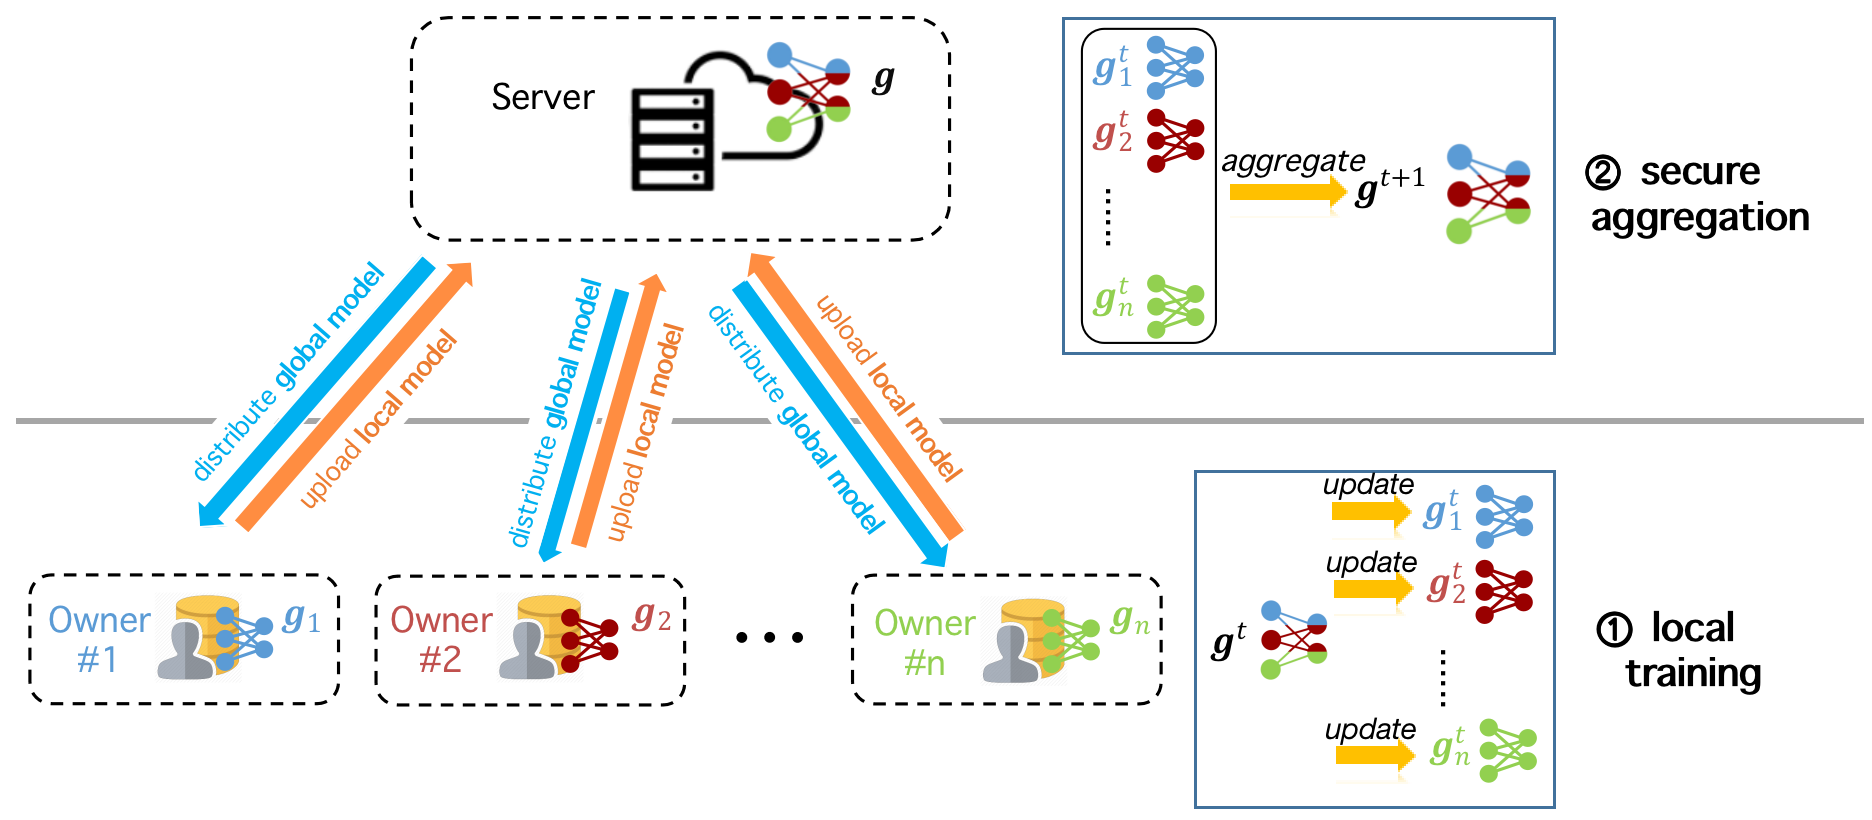
\includegraphics[width=0.85\linewidth]{submissions/YongxinTong/fig/fedavg.png}
	\caption{Workflow of federated learning over a data federation.}\label{fig:fedavg}
\end{figure}

\subsection{Local Training}\label{sec:learning-local}

In this subsection, we introduce optimizing techniques for local training from two categories, \textit{optimization through training} and \textit{optimization through data}, as follows.

\fakeparagraph{Optimization through Training}
Optimization techniques through model training are widely used in recent years. It contributes to more stable convergence and better generalization of aggregated global models.
\begin{itemize}
    \item \textbf{Regularized Loss.}
    The \textit{main idea} of regularized loss methods in federated learning is to add a regularization term to local sub-problem and is widely used for limiting local model updates and stabilizing global model.
    For example, \textsf{FedProx} \cite{Yongxin-DBLP:conf/mlsys/LiSZSTS20} proposed a regularization term to take similarity between local model and global model into account. The regularization term keeps the differences between the local and global models within a certain range.
    \textsf{FedDyn} \cite{Yongxin-DBLP:conf/iclr/AcarZNMWS21} introduces a dynamic regularization method, and ensures that the objective is dynamically updated and the local optima is close to the stationary point of the global empirical loss.
	
    \item \textbf{Extra Variable.}
    Some federated learning algorithms introduce extra variable to help improving model generalization. The \textit{main difference} between regularized loss and extra variable is that the extra variable is usually updated during local updates.
    \textsf{SCAFFOLD} \cite{Yongxin-DBLP:conf/icml/KarimireddyKMRS20} set a control variable to correct the local update moving towards the true optimum.
    Several studies \cite{Yongxin-DBLP:conf/nips/Tran-DinhPPN21, Yongxin-DBLP:conf/icde/GongLF22} introduced dual variables, converting the local object at the client side (\ie the data owner side) into a dual problem. The optimization to the dual problem contributes to automatic adaptation to global data distributions.
\end{itemize}

\fakeparagraph{Optimization through Data}
Due to statistical heterogeneity caused by non-IID data across data owners, several data-based optimization techniques were proposed to alleviate the accuracy drop of a federated learning algorithm.
\begin{itemize}
    \item \textbf{Data Augmentation.}
    Data augmentation, which enriches a dataset, is commonly used to fix the issue of non-IID data distribution on the client side to an IID one.
    \textsf{FAug} \cite{Yongxin-DBLP:journals/corr/abs-1811-11479} trained a Generative Adversarial Network (GAN) at the server and distributed the GAN to clients, where GAN could generate data to the local dataset to achieve an IID data distribution.
    \textsf{Fed-ZDAC} \cite{Yongxin-DBLP:conf/cvpr/HaoELZLCC21} proposed a zero-shot data augmentation method, which synthesized data based on the model information (only) without sharing data with the server.
	Compared with \textsf{FAug} \cite{Yongxin-DBLP:journals/corr/abs-1811-11479}, \textsf{Fed-ZDAC} \cite{Yongxin-DBLP:conf/cvpr/HaoELZLCC21} achieved a higher privacy preservation level.
	
    \item \textbf{Data Source Selection.}
    During the training process of federated learning, some data owners may hold extremely skewed data, which may lead to slow and unstable convergence of the global model.
    The \textit{main idea} of data source selection is to select proper data owners to participate the training, which alleviates the influence brought by skewed datasets.
    For instance, \textsf{FDSS} \cite{Yongxin-DBLP:conf/dasfaa/ZhangWZRTX22} observed the data source selection problem from the perspective of submodular optimization. By combining lazy evaluation and approximation of aggregated models with greedy selection, \textsf{FDSS} ensured a constant approximation ratio.
    \textsf{Oort} \cite{Yongxin-DBLP:conf/osdi/LaiZMC21} modeled selecting data owners as a multi-armed bandit problem, and improved the time-to-accuracy performance of training procedure.
\end{itemize}

\subsection{Secure Aggregation}\label{sec:learning-secure}
While local training optimization contributes to better generalization and convergence, techniques of secure aggregation are important as well for satisfying the security constraint.
Techniques of secure aggregation in federated learning can be categorized into two kinds, \textit{secure multi-party computation (SMC) based solution} and \textit{differential privacy (DP) based solution}.

\fakeparagraph{SMC based Solution}
Secure multi-party computation (SMC) enables several participants to collaboratively compute without revealing their data to each other.
When the number of data owners is large, some SMC techniques, such as garbled circuit (GC) and oblivious transfer (OT), could be inefficient for secure aggregation in federated learning.
Under this setting, efficient SMC based solutions are secret sharing (SS) and homomorphic encryption (HE).
\begin{itemize}
    \item \textbf{Secret Sharing.}
    In a secret sharing scheme, a secret consists of multiple shares and can be re-constructed only when there is a sufficient number of shares.
    When secret sharing is used in a federated learning framework, the gradients of each data owner represent a secret and are re-constructed on the server side only when enough gradients are uploaded.
    Bonawitz \etal \cite{Yongxin-DBLP:conf/ccs/BonawitzIKMMPRS17} presented a protocol to securely compute the sum of vectors, which has been used in federated learning.
	This protocol permits the server to securely average updates uploaded by data owners without leaking these updates.
    By this way, secret sharing is commonly seen in federated learning algorithms \cite{Yongxin-DBLP:conf/icics/DongCSW19, Yongxin-DBLP:journals/tifs/XuLL0L20, Yongxin-DBLP:conf/bigdataconf/SharmaXLK19} to protect the data privacy.
	
    \item \textbf{Homomorphic Encryption.}
    Homomorphic encryption guarantees security by conducting the calculation in ciphertext, and the result after decryption is same as that in plaintext calculation.
	For homomorphic encryption based secure aggregation in federated learning, data owners encrypt their local models and send them back to the server for later aggregation in ciphertext. Then, data owners decrypt the received global model and update local gradients.
    Several studies \cite{Yongxin-DBLP:journals/tifs/PhongAHWM18, Yongxin-DBLP:conf/globecom/ZhangCYD19, Yongxin-DBLP:journals/expert/ChenQWYG20, Yongxin-zhangtkde23} have adopted homomorphic encryption in the federated learning framework.
    \textsf{BatchCrypt} \cite{Yongxin-DBLP:conf/usenix/ZhangLX00020} introduced a batch encryption based technique to reduce the encryption and communication overhead caused by homomorphic encryption. It encodes a batch of gradients into a long integer data type to replace the original full precision encryption.
\end{itemize}

\fakeparagraph{DP based Solution}
Differential privacy (DP) protects privacy by adding perturbations to data. Compared with SMC, DP based solution is computationally more efficient. Thus, DP is widely used in federated learning to improve the efficiency.
Existing DP based solution in federated learning can be mainly classified into two kinds, \textit{central differential privacy (CDP)} and \textit{local differential privacy (LDP)}.

\begin{itemize}
    \item \textbf{Central Differential Privacy.}
    Central differential privacy provides a security guarantee by adding perturbation to the aggregated model on the server side. For example, Geyer \etal \cite{Yongxin-DBLP:journals/corr/abs-1712-07557} proposed a central differential privacy based method.
    During the training stage, data owners update their model weights and upload parameters to the server.
    The server then aggregates model parameters with Gaussian noise.
    Based on a similar idea, Shi \etal~\cite{Yongxin-is20shi} applied the central differential privacy to topic modeling, and \textsf{NbAFL} \cite{Yongxin-DBLP:journals/tifs/WeiLDMYFJQP20} added perturbation to local gradients in the meantime, and was shown to protect data owners from an untrusted server that planned to steal the gradients.
	
    \item \textbf{Local Differential Privacy.}
    By contrast, the local differential privacy based method adds noise to model parameters on the client side, such that model parameters can be prevented from being inferred by adversaries.
    For instance, Bao \etal \cite{Yongxin-DBLP:journals/pvldb/BaoZXYOTA22} proposed a novel local differential privacy based federated learning framework, which injects noise from shifted symmetric Skellam distributions.
	It broadened the data type of model gradients, which contributed to a lower noise level required for differential privacy.
    Local differential privacy based solutions have also been adopted in several federated learning algorithms \cite{Yongxin-DBLP:journals/tifs/WeiLDMYFJQP20, Yongxin-DBLP:conf/dasfaa/LiuCYC20, Yongxin-DBLP:conf/isit/SeifTL20, Yongxin-wangaaai20} to achieve better protection for local model parameters and more scalable efficiency.
\end{itemize}

\begin{table}[t]
\centering
\caption{Comparison of representative work on federated learning.}\label{table:comparison}

\begin{threeparttable}
\begin{tabular}{cccccc}
\toprule
Reference & \begin{tabular}[c]{@{}c@{}}Data Integration\\ Mode\end{tabular}  & \begin{tabular}[c]{@{}c@{}}Local\\ Training\end{tabular} & \begin{tabular}[c]{@{}c@{}}Secure\\ Aggregation\end{tabular} & \begin{tabular}[c]{@{}c@{}}Learning\\ Model\end{tabular} & \#(Data Owner)  \\
\midrule
\textsf{NbAFL} \cite{Yongxin-DBLP:journals/tifs/WeiLDMYFJQP20} & Horizontal & \begin{tabular}[c]{@{}c@{}}Regularized\\ Loss\end{tabular} & DP & MLP & $\le$50  \\
\textsf{SMM} \cite{Yongxin-DBLP:journals/pvldb/BaoZXYOTA22} & Horizontal & / & DP & MLP & $\le$240  \\
\textsf{FedADMM} \cite{Yongxin-DBLP:conf/icde/GongLF22} & Horizontal & \begin{tabular}[c]{@{}c@{}}Extra\\ Variable\end{tabular} & / & CNN & $\le$100  \\
\textsf{FedAvg} \cite{Yongxin-DBLP:conf/aistats/McMahanMRHA17} & Horizontal & / & / & CNN, LSTM & $\le$600 \\
\textsf{FederatedScope} \cite{Yongxin-xie2022federatedscope} & Horizontal & / & SMC, DP & CNN, GNN & $\le$260 \\
\textsf{VF2Boost} \cite{Yongxin-DBLP:conf/sigmod/FuSYJXT021} & Vertical & / & SMC & GBDT & $\le$4 \\
\textsf{Pivot} \cite{Yongxin-DBLP:journals/pvldb/WuCXCO20} & Vertical & / & SMC & GBDT & $\le$10 \\
\textsf{FTL} \cite{Yongxin-DBLP:journals/expert/LiuKXCY20} & Transfer\tnote{*} & \begin{tabular}[c]{@{}c@{}}Regularized\\ Loss\end{tabular} & SMC & AutoEncoder & $\le$2  \\
\textsf{FedHealth} \cite{Yongxin-DBLP:journals/expert/ChenQWYG20} & Transfer & \begin{tabular}[c]{@{}c@{}}Regularized\\ Loss\end{tabular} & SMC & CNN & $\le$25 \\
\bottomrule
\end{tabular}
\begin{tablenotes}
\footnotesize
\item{*} The term ``Transfer'' here represents federated transfer learning.
\end{tablenotes}


\end{threeparttable}
\end{table}

\subsection{Discussion}\label{sec:learning-discussion}
In this subsection, we give a brief introduction on the comparison of representative work in \tabref{table:comparison}.
We can observe that more studies on federated learning were studied over the horizontal data federation,
while less work studied vertical federated learning and federated transfer learning.
Moreover, we can also observe that both SMC and DP strategies are used for satisfying the security constraint. By comparison, DP based solutions tend to achieve better scalability by supporting more data owners than SMC based solution.
As shown in \figref{fig:platform}, these techniques of federated learning have been integrated into algorithm framework by industry and academia, such as FATE \cite{Yongxin-FATE}, PySyft \cite{Yongxin-PySyft}, and FederatedScope \cite{Yongxin-FederatedScope}.

\begin{figure}[t]
	\centering
    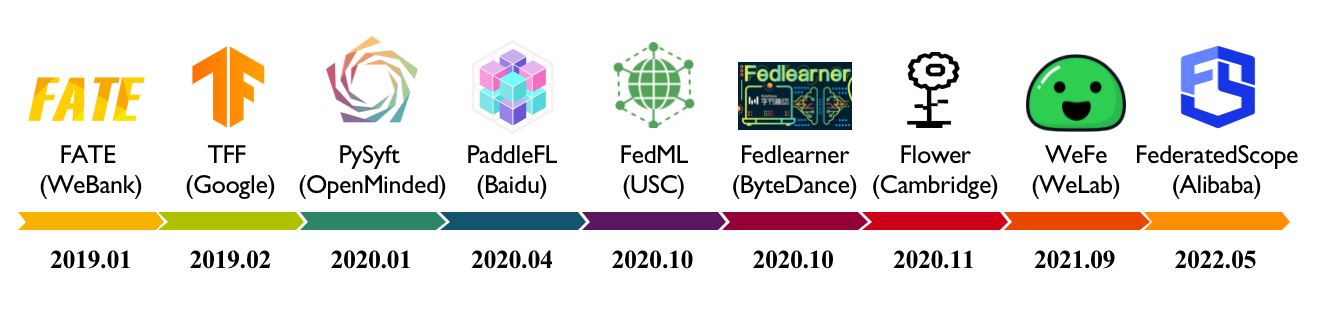
\includegraphics[width=0.95\linewidth]{submissions/YongxinTong/fig/platform.png}
	\caption{Representative frameworks for federated learning.}\label{fig:platform}
\end{figure}

\section{Future Direction}\label{sec:future}

In the following, we identify the future directions of federated computing.

\fakeparagraph{Exploring more federated queries and learning models}
To facilitate more applications on more diversified data, it will be important to explore more federated queries and federated learning models.

On one hand, as shown in \tabref{tab:data-federation-compare}, existing federated queries are mainly studied over relational data and spatial data.
Other data types, such as trajectory data and graph data, are also important for data sharing.
For example, Yuan \etal \cite{Yongxin-DBLP:journals/pvldb/YuanMWZW21} have recently proposed the concept of graph data federation, and studied subgraph matching under this setting.
Another application of graph data federation is a cross-platform ride-hailing \cite{Yongxin-DBLP:conf/kdd/WangTZRXWL22}, where each taxi company can be viewed as a data owner and their requests and passengers form a bipartite graph data federation.
As a result, Wang \etal \cite{Yongxin-DBLP:conf/kdd/WangTZRXWL22} studied how to obtain maximum weighted bipartite matching under a data federation.
Graph data federation may have other applications (\eg social networks), and many other federated graph queries have not been studied yet, which leaves a great opportunity for future research.

On the other hand, although federated learning has been widely studied in the AI and data mining community, quite a few of them ignored the issue of data security.
For instance, recent learning models, such as ViT \cite{Yongxin-DBLP:conf/iclr/DosovitskiyB0WZ21}, ResNets \cite{Yongxin-DBLP:conf/cvpr/HeZRS16}, and GraphSAGE \cite{Yongxin-DBLP:conf/nips/HamiltonYL17}, have been studied in the federated learning setting without protecting security and privacy rigorously.
What is worse, recent surveys \cite{Yongxin-DBLP:journals/csur/YinZH21} have reviewed many FL attacks such as poisoning attacks. The attacks could probe and infer sensitive information from data owners' model parameters, leading to severe privacy leakage.
Therefore, research on how to effectively defend these attacks for the aforementioned models in federated learning is still anticipated.

\fakeparagraph{Marrying Federated Queries and Federated Learning}
In the past five years, we have seen many promising results of marrying artificial intelligence (AI) and databases (DB), which is also known as DB4AI and AI4DB. One typical example of AI4DB is the concept of learned index \cite{Yongxin-DBLP:conf/sigmod/KraskaBCDP18} that uses learning models to enhance, or even replace conventional indexes like B-Trees. Another example of DB4AI is the structure-aware learning system \textsf{LMFAO} \cite{Yongxin-DBLP:journals/pvldb/Olteanu20} that decomposes the training procedure into batches of aggregate queries and further improves the efficiency by the optimization techniques of processing aggregate queries.

Motivated by these research trends, we envision that it is also possible that federated queries and federated learning could help each other.
For instance, most of existing systems for federated queries have no support for a global index, which is often used to improve the query efficiency in a distributed DBMS.
By contrast, in a data federation system for federated queries, a global index additionally needs to protect the sensitive information of all data owners.
Since there are existing studies that have shown learned indexes can reduce the index size and running time,
it might be possible that federated learning could be safely used to construct such a global index for federated queries.

\fakeparagraph{Multi-Model Federated Computing}
The variety is known as one of the fundamental challenges in managing big data.
To fit a DBMS into diversified application settings, many data models have been proposed, such as relational, spatial, key/value, and graph.
Intuitively, data-intensive applications, such as E-commerce \cite{Yongxin-DBLP:journals/csur/LuH19} and transportation \cite{Yongxin-DBLP:conf/cikm/LuHC18}, may need to manipulate and analyze data with heterogeneous data models at the same time.
Multi-model databases \cite{Yongxin-DBLP:journals/csur/LuH19} have been proposed to tackle this problem.
For example, PostgreSQL can now support several data models, including relational, key/value, JSON, XML, \etc
However, most of these studies assume that all data have been collected and stored by only one data owner.
By contrast, emerging applications have been deployed over a data federation.

On this basis, we propose a new concept called \textit{multi-model big data federated computing (``multi-model federated computing'' as short)} as the last line of future research. This computational paradigm aims to bridge the connections between data owners with diversified data models and provide joint queries and analytics while preserving data privacy/security. Under this setting, one fundamental challenge could be how to overcome the security heterogeneity \cite{Yongxin-DBLP:conf/sigmod/0012FWY20} which inherits from data model variety. To the best of our knowledge, no existing work has built such a system, which leaves a valuable opportunity for future work.

\section{Conclusion}\label{sec:conclusion}
Federated computing is a promising paradigm for data sharing, which enables secure querying and analysis across multiple autonomous data owners.
This paper introduces the fundamental concepts and general framework of federated computing, along with discussions of the challenges and related studies on federated queries and federated learning.
We also point out the future directions of federated computing and envision it as a practical solution to overcome the data isolation problem, fostering the prosperity of the information society.

\section*{Acknowledgements}
This work is partially supported by National Science Foundation of China (NSFC) under Grant No. U21A20516 and 62076017, the Beihang University Basic Research Funding No. YWF-22-L-531, and WeBank Scholars Program. Yuxiang Zeng is the corresponding author.

%\bibliographystyle{IEEEtran}
%\bibliography{ref}

% Generated by IEEEtran.bst, version: 1.14 (2015/08/26)
\begin{thebibliography}{10}
\providecommand{\url}[1]{#1}
\csname url@samestyle\endcsname
\providecommand{\newblock}{\relax}
\providecommand{\bibinfo}[2]{#2}
\providecommand{\BIBentrySTDinterwordspacing}{\spaceskip=0pt\relax}
\providecommand{\BIBentryALTinterwordstretchfactor}{4}
\providecommand{\BIBentryALTinterwordspacing}{\spaceskip=\fontdimen2\font plus
\BIBentryALTinterwordstretchfactor\fontdimen3\font minus
  \fontdimen4\font\relax}
\providecommand{\BIBforeignlanguage}[2]{{%
\expandafter\ifx\csname l@#1\endcsname\relax
\typeout{** WARNING: IEEEtran.bst: No hyphenation pattern has been}%
\typeout{** loaded for the language `#1'. Using the pattern for}%
\typeout{** the default language instead.}%
\else
\language=\csname l@#1\endcsname
\fi
#2}}
\providecommand{\BIBdecl}{\relax}
\BIBdecl

\bibitem{Yongxin-DBLP:journals/tist/YangLCT19}
Q.~Yang, Y.~Liu, T.~Chen, and Y.~Tong, ``Federated machine learning: Concept
  and applications,'' \emph{{ACM} Trans. Intell. Syst. Technol.}, vol.~10,
  no.~2, pp. 12:1--12:19, 2019.

\bibitem{Yongxin-ref_bater2017smcql}
J.~Bater, G.~Elliott, C.~Eggen, S.~Goel, A.~N. Kho, and J.~Rogers, ``{SMCQL:}
  secure query processing for private data networks,'' \emph{{PVLDB}}, vol.~10,
  no.~6, pp. 673--684, 2017.

\bibitem{Yongxin-DBLP:conf/sigmod/BharadwajC22}
A.~Bharadwaj and G.~Cormode, ``An introduction to federated computation,'' in
  \emph{{SIGMOD}}, 2022, pp. 2448--2451.

\bibitem{Yongxin-ref_tong2022hu}
Y.~Tong, X.~Pan, Y.~Zeng, Y.~Shi, C.~Xue, Z.~Zhou, X.~Zhang, L.~Chen, Y.~Xu,
  K.~Xu, and W.~Lv, ``{Hu-Fu}: Efficient and secure spatial queries over data
  federation,'' \emph{{PVLDB}}, vol.~15, no.~6, pp. 1159--1172, 2022.

\bibitem{Yongxin-DBLP:journals/pvldb/YuanMWZW21}
Y.~Yuan, D.~Ma, Z.~Wen, Z.~Zhang, and G.~Wang, ``Subgraph matching over graph
  federation,'' \emph{{PVLDB}}, vol.~15, no.~3, pp. 437--450, 2021.

\bibitem{Yongxin-DBLP:conf/aistats/McMahanMRHA17}
B.~McMahan, E.~Moore, D.~Ramage, S.~Hampson, and B.~A. y~Arcas,
  ``Communication-efficient learning of deep networks from decentralized
  data,'' in \emph{{AISTATS}}, 2017, pp. 1273--1282.

\bibitem{Yongxin-DBLP:journals/ftml/KairouzMABBBBCC21}
P.~Kairouz, H.~B. McMahan, B.~Avent, A.~Bellet, M.~Bennis, A.~N. Bhagoji, K.~A.
  Bonawitz, Z.~Charles, G.~Cormode, R.~Cummings, R.~G.~L. D'Oliveira,
  H.~Eichner, S.~E. Rouayheb, D.~Evans, J.~Gardner, Z.~Garrett,
  A.~Gasc{\'{o}}n, B.~Ghazi, P.~B. Gibbons, M.~Gruteser, Z.~Harchaoui, C.~He,
  L.~He, Z.~Huo, B.~Hutchinson, J.~Hsu, M.~Jaggi, T.~Javidi, G.~Joshi,
  M.~Khodak, J.~Kone{\v{c}}n{\'y}, A.~Korolova, F.~Koushanfar, S.~Koyejo,
  T.~Lepoint, Y.~Liu, P.~Mittal, M.~Mohri, R.~Nock, A.~{\"{O}}zg{\"{u}}r,
  R.~Pagh, H.~Qi, D.~Ramage, R.~Raskar, M.~Raykova, D.~Song, W.~Song, S.~U.
  Stich, Z.~Sun, A.~T. Suresh, F.~Tram{\`{e}}r, P.~Vepakomma, J.~Wang,
  L.~Xiong, Z.~Xu, Q.~Yang, F.~X. Yu, H.~Yu, and S.~Zhao, ``Advances and open
  problems in federated learning,'' \emph{Found. Trends Mach. Learn.}, vol.~14,
  no. 1-2, pp. 1--210, 2021.

\bibitem{Yongxin-science2016A}
T.~G.~A. for Genomics and Health, ``A federated ecosystem for sharing genomic,
  clinical data,'' \emph{Science}, vol. 352, no. 6291, pp. 1278--1280, 2016.

\bibitem{Yongxin-DBLP:conf/kdd/VaidyaC02}
J.~Vaidya and C.~Clifton, ``Privacy preserving association rule mining in
  vertically partitioned data,'' in \emph{{SIGKDD}}, 2002, pp. 639--644.

\bibitem{Yongxin-DBLP:journals/tkde/KantarciogluC04}
M.~Kantarcioglu and C.~Clifton, ``Privacy-preserving distributed mining of
  association rules on horizontally partitioned data,'' \emph{{IEEE} Trans.
  Knowl. Data Eng.}, vol.~16, no.~9, pp. 1026--1037, 2004.

\bibitem{Yongxin-DBLP:conf/sigmod/BegoliCHML18}
E.~Begoli, J.~Camacho{-}Rodr{\'{\i}}guez, J.~Hyde, M.~J. Mior, and D.~Lemire,
  ``Apache {c}alcite: {A} foundational framework for optimized query processing
  over heterogeneous data sources,'' in \emph{{SIGMOD}}, 2018, pp. 221--230.

\bibitem{Yongxin-ref_bater2018shrinkwrap}
J.~Bater, X.~He, W.~Ehrich, A.~Machanavajjhala, and J.~Rogers, ``Shrinkwrap:
  Efficient {SQL} query processing in differentially private data
  federations,'' \emph{{PVLDB}}, vol.~12, no.~3, pp. 307--320, 2018.

\bibitem{Yongxin-ref_bater2020saqe}
J.~Bater, Y.~Park, X.~He, X.~Wang, and J.~Rogers, ``{SAQE:} practical
  privacy-preserving approximate query processing for data federations,''
  \emph{{PVLDB}}, vol.~13, no.~11, pp. 2691--2705, 2020.

\bibitem{Yongxin-ref_volgushev2019conclave}
N.~Volgushev, M.~Schwarzkopf, B.~Getchell, M.~Varia, A.~Lapets, and
  A.~Bestavros, ``Conclave: secure multi-party computation on big data,'' in
  \emph{{EuroSys}}, 2019, pp. 3:1--3:18.

\bibitem{Yongxin-ref_wang2021secure}
Y.~Wang and K.~Yi, ``Secure {Y}annakakis: Join-aggregate queries over private
  data,'' in \emph{{SIGMOD}}, 2021, pp. 1969--1981.

\bibitem{Yongxin-DBLP:conf/sigmod/KraskaBCDP18}
T.~Kraska, A.~Beutel, E.~H. Chi, J.~Dean, and N.~Polyzotis, ``The case for
  learned index structures,'' in \emph{{SIGMOD}}, 2018, pp. 489--504.

\bibitem{Yongxin-DBLP:journals/pvldb/FerraginaV20}
P.~Ferragina and G.~Vinciguerra, ``The {PGM}-index: a fully-dynamic compressed
  learned index with provable worst-case bounds,'' \emph{{PVLDB}}, vol.~13,
  no.~8, pp. 1162--1175, 2020.

\bibitem{Yongxin-DBLP:conf/sigmod/DingMYWDLZCGKLK20}
J.~Ding, U.~F. Minhas, J.~Yu, C.~Wang, J.~Do, Y.~Li, H.~Zhang, B.~Chandramouli,
  J.~Gehrke, D.~Kossmann, D.~B. Lomet, and T.~Kraska, ``{ALEX:} an updatable
  adaptive learned index,'' in \emph{{SIGMOD}}, 2020, pp. 969--984.

\bibitem{Yongxin-DBLP:journals/pvldb/WuZCCWX21}
J.~Wu, Y.~Zhang, S.~Chen, Y.~Chen, J.~Wang, and C.~Xing, ``Updatable learned
  index with precise positions,'' \emph{{PVLDB}}, vol.~14, no.~8, pp.
  1276--1288, 2021.

\bibitem{Yongxin-DBLP:conf/mdm/WangFX019}
H.~Wang, X.~Fu, J.~Xu, and H.~Lu, ``Learned index for spatial queries,'' in
  \emph{{MDM}}, 2019, pp. 569--574.

\bibitem{Yongxin-DBLP:conf/vldb/0001KH20}
A.~Hadian, A.~Kumar, and T.~Heinis, ``Hands-off model integration in spatial
  index structures,'' in \emph{AIDB@VLDB}, 2020.

\bibitem{Yongxin-DBLP:conf/sigmod/Li0ZY020}
P.~Li, H.~Lu, Q.~Zheng, L.~Yang, and G.~Pan, ``{LISA:} {A} learned index
  structure for spatial data,'' in \emph{{SIGMOD}}, 2020, pp. 2119--2133.

\bibitem{Yongxin-DBLP:journals/pvldb/QiLJK20}
J.~Qi, G.~Liu, C.~S. Jensen, and L.~Kulik, ``Effectively learning spatial
  indices,'' \emph{{PVLDB}}, vol.~13, no.~11, pp. 2341--2354, 2020.

\bibitem{Yongxin-DBLP:conf/sigmod/IdreosK19}
S.~Idreos and T.~Kraska, ``From auto-tuning one size fits all to self-designed
  and learned data-intensive systems,'' in \emph{{SIGMOD}}, 2019, pp.
  2054--2059.

\bibitem{Yongxin-DBLP:journals/pvldb/MarcusKRSMK0K20}
R.~Marcus, A.~Kipf, A.~van Renen, M.~Stoian, S.~Misra, A.~Kemper, T.~Neumann,
  and T.~Kraska, ``Benchmarking learned indexes,'' \emph{{PVLDB}}, vol.~14,
  no.~1, pp. 1--13, 2020.

\bibitem{Yongxin-ref_shi2021efficient}
Y.~Shi, Y.~Tong, Y.~Zeng, Z.~Zhou, B.~Ding, and L.~Chen, ``Efficient
  approximate range aggregation over large-scale spatial data federation,''
  \emph{{IEEE} Trans. Knowl. Data Eng.}, vol.~35, no.~1, pp. 418--430, 2023.

\bibitem{Yongxin-DBLP:conf/sigmod/ChaudhuriDK17}
S.~Chaudhuri, B.~Ding, and S.~Kandula, ``Approximate query processing: No
  silver bullet,'' in \emph{{SIGMOD}}, 2017, pp. 511--519.

\bibitem{Yongxin-DBLP:journals/cacm/Lindell21}
Y.~Lindell, ``Secure multiparty computation,'' \emph{Commun. {ACM}}, vol.~64,
  no.~1, pp. 86--96, 2021.

\bibitem{Yongxin-DBLP:conf/sp/LiuWNHS15}
C.~Liu, X.~S. Wang, K.~Nayak, Y.~Huang, and E.~Shi, ``Oblivm: {A} programming
  framework for secure computation,'' in \emph{{S\&P}}, 2015, pp. 359--376.

\bibitem{Yongxin-DBLP:conf/focs/Yao82b}
A.~C. Yao, ``Protocols for secure computations (extended abstract),'' in
  \emph{{FOCS}}, 1982, pp. 160--164.

\bibitem{Yongxin-DBLP:journals/jacm/GoldreichO96}
O.~Goldreich and R.~Ostrovsky, ``Software protection and simulation on
  oblivious rams,'' \emph{J. {ACM}}, vol.~43, no.~3, pp. 431--473, 1996.

\bibitem{Yongxin-DBLP:journals/iacr/ZahurE15}
S.~Zahur and D.~Evans, ``{Obliv-C}: {A} language for extensible data-oblivious
  computation,'' \emph{{IACR} Cryptology ePrint Archive}, vol. 2015, p. 1153,
  2015.

\bibitem{Yongxin-DBLP:conf/esorics/BogdanovLW08}
D.~Bogdanov, S.~Laur, and J.~Willemson, ``Sharemind: {A} framework for fast
  privacy-preserving computations,'' in \emph{{ESORICS}}, 2008, pp. 192--206.

\bibitem{Yongxin-dasfaa23aknn}
K.~Zhang, Y.~Tong, Y.~Shi, Y.~Zeng, Y.~Xu, K.~Xu, W.~Lv, and Z.~Zheng, ``Approximate k-Nearest Neighbor Query over Spatial Data Federation,'', in \emph{{DASFAA}}, 2023, pp. 351--368.

\bibitem{Yongxin-DBLP:conf/uss/PoddarKYDPH21}
R.~Poddar, S.~Kalra, A.~Yanai, R.~Deng, R.~A. Popa, and J.~M. Hellerstein,
  ``Senate: {A} maliciously-secure {MPC} platform for collaborative
  analytics,'' in \emph{{USENIX} Security}, 2021, pp. 2129--2146.

\bibitem{Yongxin-DBLP:conf/ccs/WangRK17a}
X.~Wang, S.~Ranellucci, and J.~Katz, ``Global-scale secure multiparty
  computation,'' in \emph{{CCS}}, 2017, pp. 39--56.

\bibitem{Yongxin-ref_li2016differential}
N.~Li, M.~Lyu, D.~Su, and W.~Yang, \emph{Differential Privacy: From Theory to
  Practice}, ser. Synthesis Lectures on Information Security, Privacy, {\&}
  Trust.\hskip 1em plus 0.5em minus 0.4em\relax Morgan {\&} Claypool
  Publishers, 2016.

\bibitem{Yongxin-DBLP:journals/fcsc/ZhengWWFSLZ21}
W.~Zheng, Y.~Wu, X.~Wu, C.~Feng, Y.~Sui, X.~Luo, and Y.~Zhou, ``A survey of
  intel {SGX} and its applications,'' \emph{Frontiers Comput. Sci.}, vol.~15,
  no.~3, p. 153808, 2021.

\bibitem{Yongxin-DBLP:conf/nsdi/ZhengDBPGS17}
W.~Zheng, A.~Dave, J.~G. Beekman, R.~A. Popa, J.~E. Gonzalez, and I.~Stoica,
  ``Opaque: An oblivious and encrypted distributed analytics platform,'' in
  \emph{{NSDI}}, 2017, pp. 283--298.

\bibitem{Yongxin-DBLP:conf/mlsys/LiSZSTS20}
T.~Li, A.~K. Sahu, M.~Zaheer, M.~Sanjabi, A.~Talwalkar, and V.~Smith,
  ``Federated optimization in heterogeneous networks,'' in \emph{{MLSys}},
  vol.~2, 2020, pp. 429--450.

\bibitem{Yongxin-DBLP:conf/iclr/AcarZNMWS21}
D.~A.~E. Acar, Y.~Zhao, R.~M. Navarro, M.~Mattina, P.~N. Whatmough, and
  V.~Saligrama, ``Federated learning based on dynamic regularization,'' in
  \emph{{ICLR}}, 2021.

\bibitem{Yongxin-DBLP:conf/icml/KarimireddyKMRS20}
S.~P. Karimireddy, S.~Kale, M.~Mohri, S.~J. Reddi, S.~U. Stich, and A.~T.
  Suresh, ``{SCAFFOLD:} stochastic controlled averaging for federated
  learning,'' in \emph{{ICML}}, vol. 119, 2020, pp. 5132--5143.

\bibitem{Yongxin-DBLP:conf/nips/Tran-DinhPPN21}
Q.~Tran{-}Dinh, N.~H. Pham, D.~T. Phan, and L.~M. Nguyen, ``{FedDR} -
  randomized {Douglas-Rachford} splitting algorithms for nonconvex federated
  composite optimization,'' in \emph{NeurIPS}, 2021, pp. 30\,326--30\,338.

\bibitem{Yongxin-DBLP:conf/icde/GongLF22}
Y.~Gong, Y.~Li, and N.~M. Freris, ``{FedADMM}: {A} robust federated deep
  learning framework with adaptivity to system heterogeneity,'' in
  \emph{{ICDE}}, 2022, pp. 2575--2587.

\bibitem{Yongxin-DBLP:journals/corr/abs-1811-11479}
E.~Jeong, S.~Oh, H.~Kim, J.~Park, M.~Bennis, and S.~Kim,
  ``Communication-efficient on-device machine learning: Federated distillation
  and augmentation under non-iid private data,'' \emph{CoRR}, vol.
  abs/1811.11479, 2018.

\bibitem{Yongxin-DBLP:conf/cvpr/HaoELZLCC21}
W.~Hao, M.~El{-}Khamy, J.~Lee, J.~Zhang, K.~J. Liang, C.~Chen, and L.~Carin,
  ``Towards fair federated learning with zero-shot data augmentation,'' in
  \emph{{CVPR} Workshops}, 2021, pp. 3310--3319.

\bibitem{Yongxin-DBLP:conf/dasfaa/ZhangWZRTX22}
R.~Zhang, Y.~Wang, Z.~Zhou, Z.~Ren, Y.~Tong, and K.~Xu, ``Data source selection
  in federated learning: {A} submodular optimization approach,'' in
  \emph{{DASFAA}}, vol. 13246, 2022, pp. 606--614.

\bibitem{Yongxin-DBLP:conf/osdi/LaiZMC21}
F.~Lai, X.~Zhu, H.~V. Madhyastha, and M.~Chowdhury, ``Oort: Efficient federated
  learning via guided participant selection,'' in \emph{{OSDI}}, 2021, pp.
  19--35.

\bibitem{Yongxin-DBLP:conf/ccs/BonawitzIKMMPRS17}
K.~A. Bonawitz, V.~Ivanov, B.~Kreuter, A.~Marcedone, H.~B. McMahan, S.~Patel,
  D.~Ramage, A.~Segal, and K.~Seth, ``Practical secure aggregation for
  privacy-preserving machine learning,'' in \emph{{CCS}}, 2017, pp. 1175--1191.

\bibitem{Yongxin-DBLP:conf/icics/DongCSW19}
Y.~Dong, X.~Chen, L.~Shen, and D.~Wang, ``Privacy-preserving distributed
  machine learning based on secret sharing,'' in \emph{{ICICS}}, vol. 11999,
  2019, pp. 684--702.

\bibitem{Yongxin-DBLP:journals/tifs/XuLL0L20}
G.~Xu, H.~Li, S.~Liu, K.~Yang, and X.~Lin, ``{VerifyNet}: Secure and verifiable
  federated learning,'' \emph{{IEEE} Trans. Inf. Forensics Secur.}, vol.~15,
  pp. 911--926, 2020.

\bibitem{Yongxin-DBLP:conf/bigdataconf/SharmaXLK19}
S.~Sharma, C.~Xing, Y.~Liu, and Y.~Kang, ``Secure and efficient federated
  transfer learning,'' in \emph{{IEEE} BigData}, 2019, pp. 2569--2576.

\bibitem{Yongxin-DBLP:journals/tifs/PhongAHWM18}
L.~T. Phong, Y.~Aono, T.~Hayashi, L.~Wang, and S.~Moriai, ``Privacy-preserving
  deep learning via additively homomorphic encryption,'' \emph{{IEEE} Trans.
  Inf. Forensics Secur.}, vol.~13, no.~5, pp. 1333--1345, 2018.

\bibitem{Yongxin-DBLP:conf/globecom/ZhangCYD19}
J.~Zhang, B.~Chen, S.~Yu, and H.~Deng, ``{PEFL:} {A} privacy-enhanced federated
  learning scheme for big data analytics,'' in \emph{{GLOBECOM}}, 2019, pp.
  1--6.

\bibitem{Yongxin-DBLP:journals/expert/ChenQWYG20}
Y.~Chen, X.~Qin, J.~Wang, C.~Yu, and W.~Gao, ``{FedHealth}: {A} federated
  transfer learning framework for wearable healthcare,'' \emph{{IEEE} Intell.
  Syst.}, vol.~35, no.~4, pp. 83--93, 2020.

\bibitem{Yongxin-zhangtkde23}
Y.~Zhang, Y.~Shi, Z.~Zhou, C.~Xue, Y.~Xu, K.~Xu, and J.~Du, ``Efficient and Secure Skyline Queries over Vertical Data Federation,'' \emph{{IEEE} Trans. Knowl. Data Eng.}, pp. 1--12, 2023.

\bibitem{Yongxin-DBLP:conf/usenix/ZhangLX00020}
C.~Zhang, S.~Li, J.~Xia, W.~Wang, F.~Yan, and Y.~Liu, ``{BatchCrypt}: Efficient
  homomorphic encryption for cross-silo federated learning,'' in \emph{{USENIX}
  {ATC}}, 2020, pp. 493--506.

\bibitem{Yongxin-DBLP:journals/corr/abs-1712-07557}
R.~C. Geyer, T.~Klein, and M.~Nabi, ``Differentially private federated
  learning: {A} client level perspective,'' \emph{CoRR}, vol. abs/1712.07557,
  2017.

\bibitem{Yongxin-is20shi}
Y.~Shi, Y.~Tong, Z.~Su, D.~Jiang, Z.~Zhou, and W.~Zhang, ``Federated Topic Discovery: {A} Semantic Consistent Approach,'' \emph{{IEEE} Intell. Syst.}, vol.~36, no.5, pp. 96--103, 2021.


\bibitem{Yongxin-DBLP:journals/tifs/WeiLDMYFJQP20}
K.~Wei, J.~Li, M.~Ding, C.~Ma, H.~H. Yang, F.~Farokhi, S.~Jin, T.~Q.~S. Quek,
  and H.~V. Poor, ``Federated learning with differential privacy: Algorithms
  and performance analysis,'' \emph{{IEEE} Trans. Inf. Forensics Secur.},
  vol.~15, pp. 3454--3469, 2020.

\bibitem{Yongxin-DBLP:journals/pvldb/BaoZXYOTA22}
E.~Bao, Y.~Zhu, X.~Xiao, Y.~Yang, B.~C. Ooi, B.~H.~M. Tan, and K.~M.~M. Aung,
  ``Skellam mixture mechanism: a novel approach to federated learning with
  differential privacy,'' \emph{{PVLDB}}, vol.~15, no.~11, pp. 2348--2360,
  2022.

\bibitem{Yongxin-DBLP:conf/dasfaa/LiuCYC20}
R.~Liu, Y.~Cao, M.~Yoshikawa, and H.~Chen, ``{FedSel}: Federated {SGD} under
  local differential privacy with top-k dimension selection,'' in
  \emph{{DASFAA}}, vol. 12112, 2020, pp. 485--501.

\bibitem{Yongxin-DBLP:conf/isit/SeifTL20}
M.~Seif, R.~Tandon, and M.~Li, ``Wireless federated learning with local
  differential privacy,'' in \emph{{ISIT}}, 2020, pp. 2604--2609.

\bibitem{Yongxin-wangaaai20}
Y.~Wang, Y.~Tong, and D.~Shi, ``Federated Latent Dirichlet Allocation: {A} Local Differential Privacy
                  Based Framework,'' in \emph{{AAAI}}, 2020, pp. 6283--6290.

\bibitem{Yongxin-xie2022federatedscope}
Y.~Xie, Z.~Wang, D.~Chen, D.~Gao, L.~Yao, W.~Kuang, Y.~Li, B.~Ding, and
  J.~Zhou, ``{Federatedscope}: A flexible federated learning platform for
  heterogeneity,'' \emph{{PVLDB}}, vol.~16, no.~5, p. 1059–1072, 2022.

\bibitem{Yongxin-DBLP:conf/sigmod/FuSYJXT021}
F.~Fu, Y.~Shao, L.~Yu, J.~Jiang, H.~Xue, Y.~Tao, and B.~Cui,
  ``{VF}\({}^{\mbox{2}}\){Boost}: Very fast vertical federated gradient
  boosting for cross-enterprise learning,'' in \emph{{SIGMOD}}, 2021, pp.
  563--576.

\bibitem{Yongxin-DBLP:journals/pvldb/WuCXCO20}
Y.~Wu, S.~Cai, X.~Xiao, G.~Chen, and B.~C. Ooi, ``Privacy preserving vertical
  federated learning for tree-based models,'' \emph{{PVLDB}}, vol.~13, no.~11,
  pp. 2090--2103, 2020.

\bibitem{Yongxin-DBLP:journals/expert/LiuKXCY20}
Y.~Liu, Y.~Kang, C.~Xing, T.~Chen, and Q.~Yang, ``A secure federated transfer
  learning framework,'' \emph{{IEEE} Intell. Syst.}, vol.~35, no.~4, pp.
  70--82, 2020.

\bibitem{Yongxin-FATE}
``{FATE},'' \url{https://github.com/FederatedAI/FATE}, last accessed 28 Feb
  2023.

\bibitem{Yongxin-PySyft}
``{PySyft},'' \url{https://github.com/OpenMined/PySyft}, last accessed 28 Feb
  2023.

\bibitem{Yongxin-FederatedScope}
``{FederatedScope},'' \url{https://github.com/alibaba/FederatedScope}, last
  accessed 28 Feb 2023.

\bibitem{Yongxin-DBLP:conf/kdd/WangTZRXWL22}
Y.~Wang, Y.~Tong, Z.~Zhou, Z.~Ren, Y.~Xu, G.~Wu, and W.~Lv, ``{Fed-LTD}:
  Towards cross-platform ride hailing via federated learning to dispatch,'' in
  \emph{{SIGKDD}}, 2022, pp. 4079--4089.

\bibitem{Yongxin-DBLP:conf/iclr/DosovitskiyB0WZ21}
A.~Dosovitskiy, L.~Beyer, A.~Kolesnikov, D.~Weissenborn, X.~Zhai,
  T.~Unterthiner, M.~Dehghani, M.~Minderer, G.~Heigold, S.~Gelly, J.~Uszkoreit,
  and N.~Houlsby, ``An image is worth 16x16 words: Transformers for image
  recognition at scale,'' in \emph{{ICLR}}, 2021.

\bibitem{Yongxin-DBLP:conf/cvpr/HeZRS16}
K.~He, X.~Zhang, S.~Ren, and J.~Sun, ``Deep residual learning for image
  recognition,'' in \emph{{CVPR}}, 2016, pp. 770--778.

\bibitem{Yongxin-DBLP:conf/nips/HamiltonYL17}
W.~L. Hamilton, Z.~Ying, and J.~Leskovec, ``Inductive representation learning
  on large graphs,'' in \emph{{NeurIPS}}, 2017, pp. 1024--1034.

\bibitem{Yongxin-DBLP:journals/csur/YinZH21}
X.~Yin, Y.~Zhu, and J.~Hu, ``A comprehensive survey of privacy-preserving
  federated learning: {A} taxonomy, review, and future directions,''
  \emph{{ACM} Comput. Surv.}, vol.~54, no.~6, pp. 131:1--131:36, 2022.

\bibitem{Yongxin-DBLP:journals/pvldb/Olteanu20}
D.~Olteanu, ``The relational data borg is learning,'' \emph{{PVLDB}}, vol.~13,
  no.~12, pp. 3502--3515, 2020.

\bibitem{Yongxin-DBLP:journals/csur/LuH19}
J.~Lu and I.~Holubov{\'{a}}, ``Multi-model databases: {A} new journey to handle
  the variety of data,'' \emph{{ACM} Comput. Surv.}, vol.~52, no.~3, pp.
  55:1--55:38, 2019.

\bibitem{Yongxin-DBLP:conf/cikm/LuHC18}
J.~Lu, I.~Holubov{\'{a}}, and B.~Cautis, ``Multi-model databases and tightly
  integrated polystores: Current practices, comparisons, and open challenges,''
  in \emph{{CIKM}}, 2018, pp. 2301--2302.

\bibitem{Yongxin-DBLP:conf/sigmod/0012FWY20}
Y.~Cao, W.~Fan, Y.~Wang, and K.~Yi, ``Querying shared data with security
  heterogeneity,'' in \emph{{SIGMOD}}, 2020, pp. 575--585.

\end{thebibliography}

\end{document} 